% !TeX root = main.tex

%\setkeys{Gin}{draft}

\onehalfspacing
\section{Lab Assignment Goals}
\vspace{.35cm}
\justifying 

This objective of this lab assignment was to methodically evaluate a common source amplifier built with the ALD1105 MOSFET, with the overarching objective of determining how variations in load resistance and signal generator resistance affect circuit performance. The group’s tasks were organized into a series of experiments, each aimed at addressing distinct aspects of amplifier behavior.
In the first experiment, the DC operating point was established by adjusting the DC bias voltage $V_G$ until the output voltage $V_O$ reached $5$V. This step involved measuring node voltages and calculating the corresponding drain currents, providing a baseline for subsequent analysis. Establishing an accurate operating point is critical to ensure that the MOSFET operates in the intended region, which is a fundamental concept that can sometimes be overlooked in traditional electrical engineering coursework.
This experiment was intended to highlight the impact of how very slight adjustments to load resistance, along with signal generator resistance, will result in large changes with the output impedance and thus have a larger affect upon the overall stability of the circuit. 

\vspace{.35cm}

\begin{center}
\begin{figure}[ht]
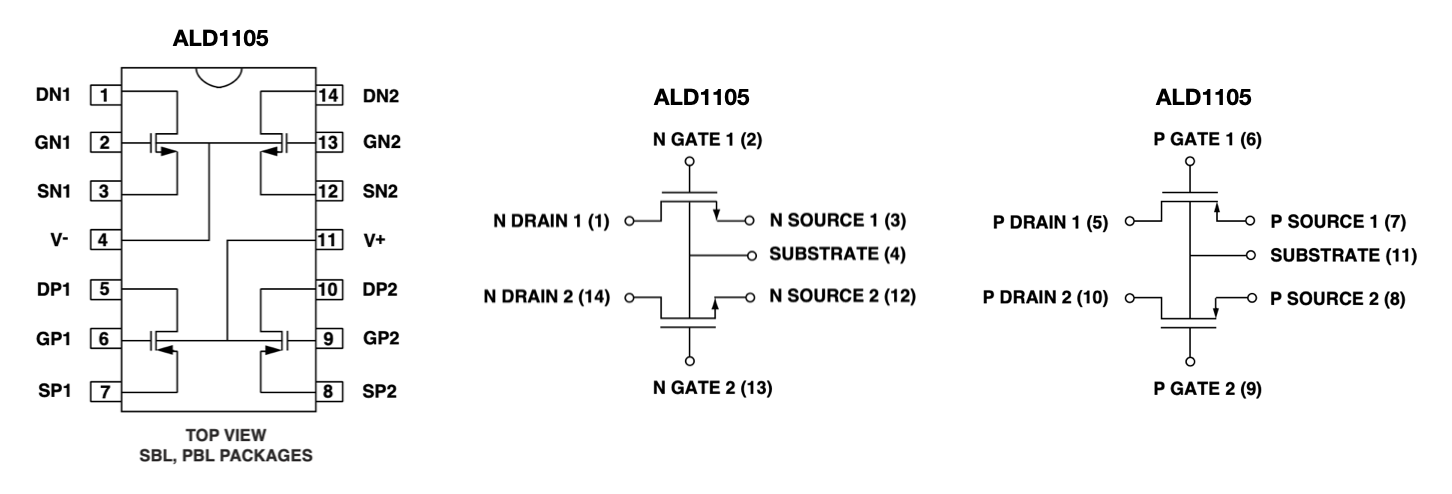
\includegraphics[scale=0.5\linewidth]{Chapter_3/Lab_03_Image_1.png}
\vspace{.55cm}
\caption{The pinout and block diagram of the ALD1105, \textbf{Note: $V^{-}$ is the body of the NMOS devices which is connected to lowest potential and $V^{+}$ is the body of the PMOS devices which is connected to the highest potential. }}
\label{Ch3_fig:1}
\end{figure}
\end{center}

\newpage

\section{Experiment 1: DC Operating Point}

Using the circuit shown below with the parameter values given, adjust the DC voltage $V_{GG}$ such that the output voltage $V_{O}$ = 5 V

\begin{itemize}

\item Find the dc operating point by measuring the node voltages and calculating the currents. Complete the summary table. 
	
\end{itemize}

\begin{center}
\begin{circuitikz}[american]
\ctikzset{tripoles/mos style=arrows}

\draw

(-4,2) node[pmos,scale=2,xscale=-1] (Q3) {}
(4,2) node[pmos,scale=2] (Q2) {}
(4,-3) node[nmos,scale=2] (Q1) {}
(Q3.center) node[left] {$Q_{3}$}
(Q2.center) node[right] {$Q_{2}$}
(Q1.center) node[right] {$Q_{1}$}
(Q3.S) node[vdd] (vdd) {$+V_{DD}$}
(Q3.D) to[R=$R$] ++(0,-3) node[ground] {}
(Q3.D) to[short,*-] ++(2.5,0) to[short,-*] ++(0,1.53)
(Q3.G) -- (Q2.G)
(Q2.S) node[vdd] (vdd) {$+V_{DD}$}
(Q1.S) node[ground] {}
(Q2.D) -- (Q1.D)
(Q1.G)  to[C=$C_{B}$] ++(-2,0) to[R=$R_{sig}$] ++(-2,0) to[vsource,l=$v_{sig}$] ++(0,-3) node[ground] {}
(Q1.G) to[R=$R_{G}$,*-] ++(0,2) node[vdd] (vdd) {$+V_{G}$}
(Q1.D) to[open] ++(0,1) node[left] {$V_{O}$}
(Q1.D) to[open] ++(0,1) to[C=$C_{B}$,*-] ++(3,0) to[R=$R_{L}$,v=$v_{o}$] ++(0,-3) node[ground] {}
;
\end{circuitikz}
\end{center}
\begin{center}
\vspace{1cm}
$V_{DD} = 10$ V \hspace{.5cm} $ V_{O} = 5$ V \hspace{.5cm} $C_{B} = 0.1 \mu$ F \\
\vspace{.2cm}
$R = 15$k $\Omega$  \hspace{.5cm} $R_{G} =10$M $\Omega$  \\
\vspace{.2cm}
$K_{N} = 270 \hspace{.25cm} \mu$A/V$^2$ \hspace{.25cm} $V_{T_n} = 0.573$ V \hspace{.25cm} $\lambda_{N} = 0.0165   $V$^{-1}$ \\
\vspace{.2cm}
$K_{P} = 88 \hspace{.15cm}  \mu$A/V$^2$ \hspace{.05cm} $V_{Tp} = -0.647$\hspace{.15cm}V \hspace{.25cm} $\lambda_{P} = 0.0219$  V$^{-1}$ \\
\vspace{.2cm}
\end{center}
\begin{center}
\begin{figure}[ht]
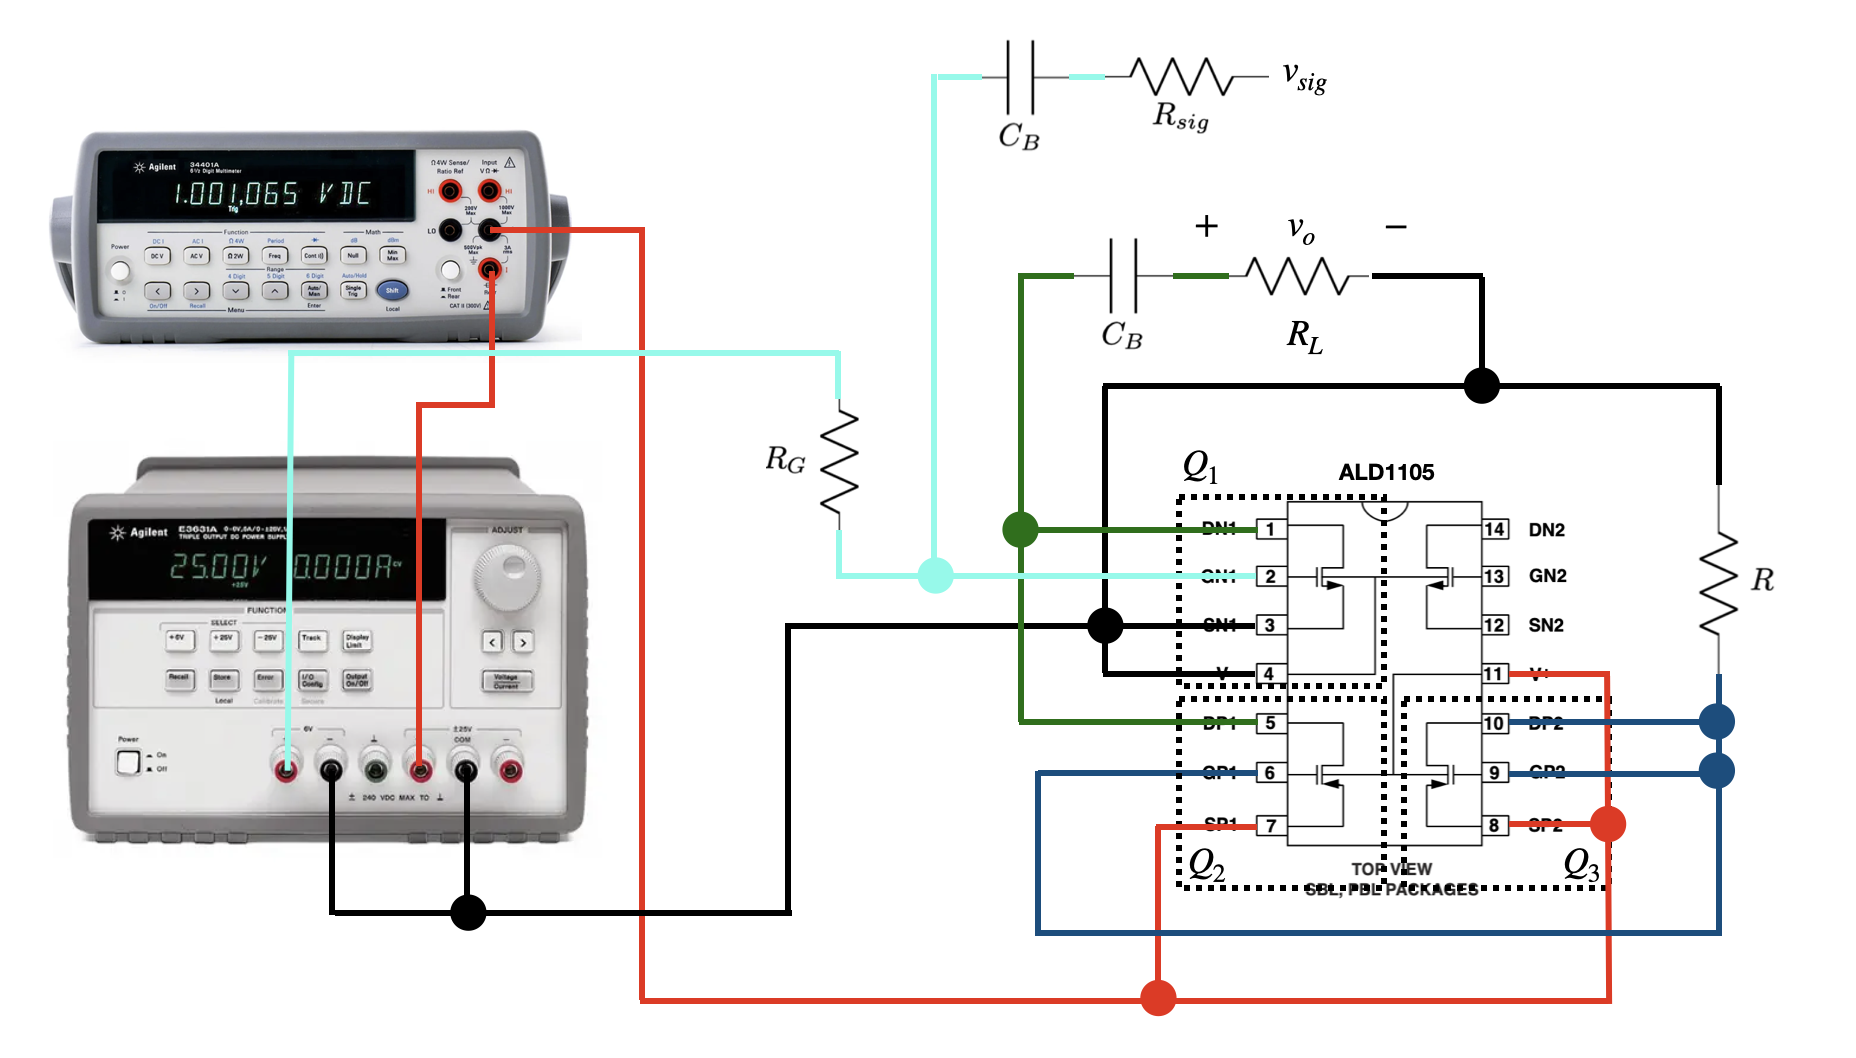
\includegraphics[scale=0.45]{Chapter_3/Lab_03_Image_2.png}
\caption{\emph{Wiring diagram of the Common Source Amplifier.}}
\label{Ch3_fig:2}
\end{figure}
\end{center}

\newpage

\vspace{.25cm}

\subsection{Measurement Issues \& 60 Hz Noise}

The physical measurement data were compromised due to improper grounding practices. In this instance, the use of separate ground rails resulted in ground loops that injected considerable $60$ Hz interference into the circuit measurements. This phenomenon is particularly problematic with the ALD1105 MOSFET, as its performance is highly sensitive to noise in the biasing network. Wiring the transistor to multiple different rails will result in ground loops that introduce significant $60$ Hz interference into measurement data, which this experiment demonstrated quite clearly. \cite{yao2015ecce}

In this scenario, the use of separate ground rails for the DC power supply, circuit, oscilloscope probes, and function generator led to mismatched ground potentials. According to an IEEE article on mitigating noise in electronic measurement systems, improper grounding practices can lead to the formation of ground loops that introduce significant $60 Hz$ interference into measurement data. In this case, using separate ground rails for the DC power supply, circuit, oscilloscope probes, and function generator resulted in mismatched ground potentials. This is particularly problematic when working with the ALD1105 MOSFET, which is highly sensitive to noise in its biasing network and operating conditions. \cite{cavache2023siitme}

\newpage
\section{Experiment 2: Investigating the Role of \texorpdfstring{$R_{sig}$}{Rsig}}

After establishing the DC operating point in Experiment 1, the role of the signal generator resistance, \(R_{sig}\), on the overall AC small-signal gain, \(G_v\), was investigated. The gain was defined as:

\[
G_v = \frac{v_o}{v_{sig}}
\]

The following procedure was implemented:

\begin{itemize}
    \item The load resistance was set to \(R_{L} = 10\,\text{M}\Omega\) (as provided by the oscilloscope probe).
    \item The small-signal gain, \(G_v\), was measured for various values of \(R_{sig}\), specifically for:
\end{itemize}
\vspace{0.2cm}
\begin{center}
\(R_{sig} = 10\,\text{M}\Omega\) \\[0.2cm]
\(R_{sig} = 100\,\text{k}\Omega\) \\[0.2cm]
\(R_{sig} = 10\,\text{k}\Omega\) \\[0.2cm]
\(R_{sig} = 1\,\text{k}\Omega\)
\end{center}


\section{Experiment 3: Investigating the Role of \texorpdfstring{$R_{L}$}{RL}}

Following the establishment of the DC operating point in Experiment 1, the influence of the load resistance, \(R_{L}\), on the AC small-signal gain, \(G_v\), was examined. The gain was defined as:

\[
G_v = \frac{v_o}{v_{sig}}
\]

The following procedure was executed:

\begin{itemize}
    \item The signal generator resistance was fixed at \(R_{sig} = 1\,\text{k}\Omega\).
    \item The small-signal gain, \(G_v\), was measured for various values of \(R_{L}\), specifically:
\end{itemize}
\vspace{0.2cm}
\begin{center}
\(R_{L} = 10\,\text{M}\Omega\) \\[0.2cm]
\(R_{L} = 100\,\text{k}\Omega\) \\[0.2cm]
\(R_{L} = 10\,\text{k}\Omega\) \\[0.2cm]
\(R_{L} = 1\,\text{k}\Omega\)
\end{center}

\section{Post Lab Data Analysis}

The post-lab analysis consisted of the following tasks:

\begin{itemize}

\item Simulate the circuits from experiments 1, 2, and 3 following the same procedure of sweeping $V_{GG}$ to find the bias point where $V_{O} = 5$V for experiment 1. Then operating under the bias condition, perform an AC analysis to find the ac small signal gain $G_{V}$ under the various $R_{sig}$ and $R_{L}$ conditions specified in experiments 2 and 3. 
\item The completed simulated data been entered into the tables, (\emph{the missing measurements will completed before the next lab meeting}), as specified below:
	
\end{itemize}

\begin{center}
	\begin{table}[H]
	\centering
	\renewcommand{\arraystretch}{1.0}
	\begin{tabular}{ | >{\centering\arraybackslash} m{2.5cm} | >{\centering\arraybackslash} m{2.5cm} | >{\centering\arraybackslash} m{2.5cm} | >{\centering\arraybackslash} m{2.5cm} | >{\centering\arraybackslash} m{2.5cm} | }
	\hline
	\multicolumn{5}{|c|}{\textbf{Experiment 1 Summary Table}} \\ \hline
	\textbf{Device} & \textbf{Quantity} & \textbf{Simulated} &\textbf{Measured} & \textbf{Units} \\ \hline
		\multirow{5}{*}{\(Q_1\)} 
		& \(I_{D}\)    & \(494.0\)  & $485.000$ & $\mu$A \\ \cline{2-5}
		& \(|V_{OV}|\) & \(1.299\)  & $1.290$ & V  \\ \cline{2-5}
		& \(V_{G}\)    & \(1.872\)  & $1.860$ & V  \\ \cline{2-5}
		& \(V_{D}\)    & \(5.058\)  & $4.970$ & V  \\ \cline{2-5}
		& \(V_{S}\)    & \(0.000\)  & $0.000$ & V  \\ \hline
		\multirow{5}{*}{\(Q_2\)}
		& \(I_{D}\)    & \(494.0\)  & $-480.000$ & $\mu$A \\ \cline{2-5}
		& \(|V_{OV}|\) & \(7.481\)  & $2.310$ & V \\ \cline{2-5}
		& \(V_{G}\)    & \(1.872\)  & $7.030$ & V \\ \cline{2-5}
		& \(V_{D}\)    & \(5.058\)  & $4.970$ & V \\ \cline{2-5}
		& \(V_{S}\)    & \(10.000\) & $9.990$ & V \\ \hline
		\multirow{5}{*}{\(Q_3\)}
		& \(I_{D}\)    & \(494.0\)  & $-480.009$ & $\mu$A \\ \cline{2-5}
		& \(|V_{OV}|\) & \(2.250\)  & $2.310$ & V \\ \cline{2-5}
		& \(V_{G}\)    & \(7.103\)  & $7.040$ & V \\ \cline{2-5}
		& \(V_{D}\)    & \(7.103\)  & $7.040$ & V \\ \cline{2-5}
		& \(V_{S}\)    & \(10.000\) & $9.99$ & V \\ \hline
	\end{tabular}
	\caption{Experiment 1 Summary Table}
	\end{table}
\end{center}

\newpage
\begin{center}
	\begin{table}[H]
	\renewcommand{\arraystretch}{1.2}
	\begin{tabular}{ | >{\centering\arraybackslash} m{3.5cm} | >{\centering\arraybackslash} m{2.5cm} | >{\centering\arraybackslash} m{2.5cm} | >{\centering\arraybackslash} m{2.5cm} | >{\centering\arraybackslash} m{2cm} | }
	\hline
	\multicolumn{5}{|c|}{\textbf{AC Small Signal Gain \(R_{L}=10\,\text{M} \Omega\)}} \\ \hline
	Condition & Quantity & Simulated  & Measured & Units \\ \hline
	\multirow{2}{*}{\(R_{sig}=10\,\text{M}\Omega\)} 
	 & \(G_{v}\)  & \(-21.900\)  & \(7.6110\)  & V/V   \\ \cline{2-5} 
	 & \(G_{v}\)  & \(26.810\)   & \(17.6288\)  & dB \\ \hline
	\multirow{2}{*}{\(R_{sig}=100\,\text{k}\Omega\)} 
	 & \(G_{v}\)  & \(-43.365\)  & \(16.2100\)  & V/V   \\ \cline{2-5} 
	 & \(G_{v}\)  & \(32.743\)   & \(24.1957\)  & dB \\ \hline
	\multirow{2}{*}{\(R_{sig}=10\,\text{k}\Omega\)} 
	 & \(G_{v}\)  & \(-43.756\)  & \(20.1700\)  & V/V   \\ \cline{2-5} 
	 & \(G_{v}\)  & \(32.821\)   & \(26.0941\)  & dB \\ \hline
	\multirow{2}{*}{\(R_{sig}=1\,\text{k}\Omega\)} 
	 & \(G_{v}\)  & \(-43.795\)  & \(22.3100\)  & V/V   \\ \cline{2-5} 
	 & \(G_{v}\)  & \(32.829\)   & \(26.9700\)  & dB \\ \hline
	\end{tabular}
	\caption{Experiment 2 Summary Table}
	\end{table}
\end{center}

\begin{figure}[H]
	\centering
	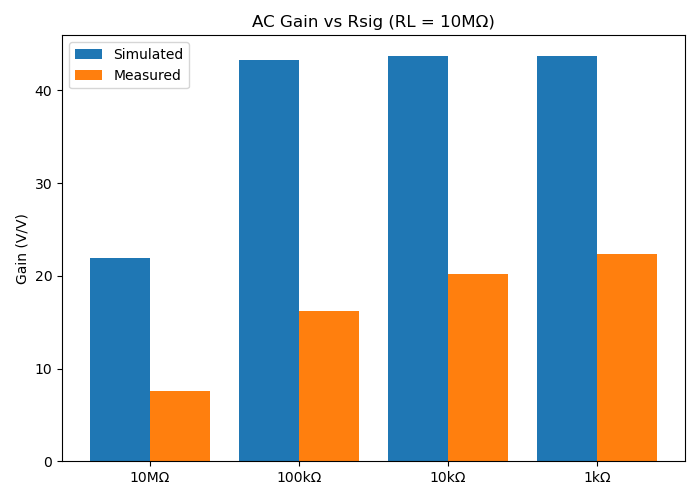
\includegraphics[width=0.75\linewidth]{Chapter_3/Lab_03_RL_10_Mohm.png}
	\caption{Simulated vs Measured data for $R_L = 10~\mathrm{M\Omega}$}
	\label{Ch3_fig:3}
\end{figure}

\newpage
\begin{center}
	\begin{table}[H]
	\centering
	\renewcommand{\arraystretch}{1.2}
		\begin{tabular}{ | >{\centering\arraybackslash} m{3.5cm} | >{\centering\arraybackslash} m{2.5cm} | >{\centering\arraybackslash} m{2.5cm} | >{\centering\arraybackslash} m{2.5cm} | >{\centering\arraybackslash} m{2cm} | }
		\hline
		\multicolumn{5}{|c|}{\textbf{AC Small Signal Gain \(R_{sig}=1\,\text{k} \Omega\)}} \\ \hline
		Condition & Quantity & Simulated  & Measured & Units \\ \hline
		\multirow{2}{*}{\(R_{L}=10\,\text{M}\Omega\)} 
		    & \(G_{v}\)  & \(-21.900\)  & \(31.2000\)  & V/V   \\ \cline{2-5} 
		    & \(G_{v}\)  & \(26.810\)   & \(20.881\)  & dB \\ \hline
		\multirow{2}{*}{\(R_{L}=100\,\text{k}\Omega\)} 
		    & \(G_{v}\)  & \(-13.943\)  & \(23.5000\)  & V/V   \\ \cline{2-5} 
		    & \(G_{v}\)  & \(22.887\)   & \(27.4214\)  & dB \\ \hline
		\multirow{2}{*}{\(R_{L}=10\,\text{k}\Omega\)} 
		    & \(G_{v}\)  & \(-3.240\)   & \(3.6500\)  & V/V   \\ \cline{2-5} 
		    & \(G_{v}\)  & \(10.211\)   & \(11.2459\)  & dB \\ \hline
		\multirow{2}{*}{\(R_{L}=1\,\text{k}\Omega\)} 
		    & \(G_{v}\)  & \(-0.373\)   & \(0.9510\)  & V/V   \\ \cline{2-5} 
		    & \(G_{v}\)  & \(-8.555\)   & \(-0.4364\)  & dB \\ \hline
		\end{tabular}
	\caption{Experiment 3 Summary Table}
	\end{table}	
\end{center}

\begin{figure}[H]
	\centering
	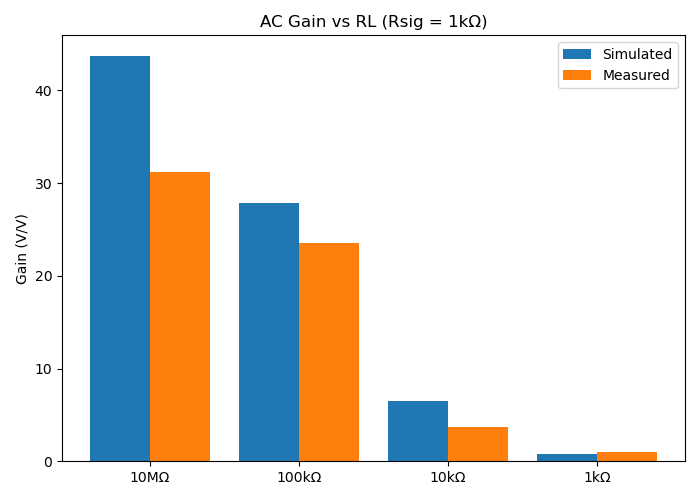
\includegraphics[width=0.75\linewidth]{Chapter_3/Lab_03_Rsig_1kohm.png}
	\caption{Simulated vs Measured data for $R_{\text{sig}} = 1~\mathrm{k\Omega}$}
	\label{Ch3_fig:4}
\end{figure}

\section{Code Listings}

The Python code used for the common source amplifier analysis can be found in the Appendix: Common Source Amp LTSpice Sweep (\cref{lst:Ch3:List1}).

\section{Conclusion}
\singlespacing
This lab successfully demonstrated the critical influence of source and load resistances on the performance of a common source amplifier using the ALD1105 MOSFET. Through a series of controlled experiments, both simulated and measured, the impact of varying $R_{sig}$​​ and $R_{L}$​​ on the AC small-signal gain $G_{V}$​ was thoroughly evaluated.

In Experiment 1, the DC operating point was accurately established by adjusting $V_{O}$​ such that the output voltage $V_{O}$ was $5$ V. This step confirmed the theoretical behavior of MOSFETs in the saturation region and emphasized the importance of correct biasing for reliable amplifier operation. The lack of close agreement between simulated and measured data reinforced the inaccuracy of the transistor model.

Experiment 2 showed that as $R_{sig}$​​ ​ decreased, the voltage gain $G_v$​ increased significantly, particularly in the measured results. This outcome is consistent with theoretical expectations, as a lower source resistance reduces signal attenuation before the gate of the MOSFET, allowing a greater portion of the input signal to modulate the channel current.
 
Experiment 3 revealed a strong dependence of gain on the load resistance $R_{L}$​​. Higher values of $R_{L}$​ led to markedly high gains, again matching theoretical predictions based on the amplifier’s gain formula $G_v \approx -g_m R_D \parallel R_L$​.  Results emphasized that loading effects from external measurement equipment (e.g., oscilloscope probes) or downstream circuitry can significantly influence observed performance.

The major insight from the lab was effects of grounding practices on measurement quality. Ground loops introduced substantial 60 Hz noise, initially preventing accurate gain readings. Once corrected, the improved grounding scheme allowed for reliable data collection that matched simulation trends closely. This lab demonstrated the sensitivity of analog circuits to parasitics and component values, especially in high-impedance configurations. Importance of thoughtful design and measurement practices is paramount for achieving predictable amplifier behavior.

\clearpage
\printbibliography[heading=subbibliography]